	\section{Technical Analysis and Proofs}
	\label{sec:technical}
	
	This section provides the mathematical backbone of our main results. We begin by constructing the implicit kernels induced by the transformer architecture, then analyze the gradient flow dynamics, and finally synthesize these to explain the emergence of implicit regularization and its phase transition. Detailed, step-by-step proofs of Theorems 1–3 are deferred to Appendix B, while here we present the key lemmas and conceptual flow.
	
	\subsection{Explicit Kernel Construction and Properties}
	\label{subsec:kernels}
	
	The first step is to understand what kind of kernel a single transformer block implicitly defines when trained with gradient flow.
	
	\subsubsection{The Attention Kernel $K_{\text{att}}$}
	\label{subsubsec:att_kernel}
	
	Consider the attention output for a query token $q$ and key tokens $\{k_i\}$. Under random initialization of $W_Q, W_K$, the attention weights before softmax are Gaussian processes. In the infinite-width limit for the attention heads (or via a linearization argument), the expectation of the attention mechanism leads to a deterministic kernel.
	
	\begin{lemma}[Attention Kernel]
		\label{lem:att_kernel}
		Let $W_Q, W_K \sim \mathcal{N}(0, \sigma_q^2 I)$, $W_V = I$, $W_O = I$ for simplicity (analysis extends to general case). For query $q$ and key $k$ in $\R^d$, the expected attention weight (ignoring the value transformation for the kernel definition) under the linearized softmax approximation is:
		\[
		K_{\text{att}}(q, k) = \exp\left(\frac{\inner{q}{A k}}{\tau}\right),
		\]
		where $A = \sigma_q^2 I$ is a positive semi-definite matrix, and $\tau = \sqrt{d}$ is the temperature scaling. In general, $A = \mathbb{E}[W_Q W_K\trans]$ reflects the alignment between query and key projections learned during pre-training.
	\end{lemma}
	
	\begin{proof}[Sketch]
		The dot-product $\frac{1}{\sqrt{d}} q\trans W_Q\trans W_K k$ is a zero-mean Gaussian with variance $\sigma_q^4 (q\trans k)^2 / d$. Using the Taylor expansion of softmax and taking expectation over the Gaussian weights, we obtain the exponential form. The full proof accounts for the normalization across keys and is given in Appendix B.1.
	\end{proof}
	
	\textbf{Properties:}
	\begin{itemize}
		\item $K_{\text{att}}$ is a \textit{positive definite} kernel (an exponential of a linear kernel).
		\item It is highly \textit{non-stationary} and sensitive to the norm of inputs.
		\item Its spectrum decays rapidly. For inputs drawn from $\mathcal{N}(0, \Sigma)$, the eigenvalues $\mu_i^{\text{att}}$ of the integral operator associated with $K_{\text{att}}$ satisfy $\mu_i^{\text{att}} \leq C \exp(-\gamma i)$, where $\gamma$ depends on $\Sigma$ and $A$.
	\end{itemize}
	
	\subsubsection{The MLP Kernel $K_{\text{mlp}}$}
	\label{subsubsec:mlp_kernel}
	
	For the MLP with ReLU activation, we leverage the Neural Tangent Kernel (NTK) theory.
	
	\begin{lemma}[ReLU NTK for MLP]
		\label{lem:mlp_kernel}
		Consider the two-layer MLP $f_{\text{mlp}}(x) = \frac{1}{\sqrt{m}} W_2 \sigma(W_1 x)$, with $W_1 \in \R^{m \times d} \sim \mathcal{N}(0,1)$, $W_2 \in \R^{1 \times m} \sim \mathcal{N}(0,1)$, and $\sigma(z)=\max(0,z)$. In the limit $m \to \infty$, the NTK of this MLP is:
		\[
		K_{\text{mlp}}(x, z) = \frac{1}{\pi} \left[ \norm{x} \norm{z} (\sin \theta_{xz} + (\pi - \theta_{xz}) \cos \theta_{xz}) \right],
		\]
		where $\theta_{xz} = \arccos\left(\frac{\inner{x}{z}}{\norm{x}\norm{z}}\right)$ is the angle between $x$ and $z$.
	\end{lemma}
	
	\begin{proof}
		This is a standard result \citep{arora2019exact}. The NTK is the sum of the kernels from the first and second layers. For ReLU, the closed-form expression involves the angle between inputs. See Appendix B.2 for derivation tailored to our architecture.
	\end{proof}
	
	\textbf{Properties:}
	\begin{itemize}
		\item $K_{\text{mlp}}$ is \textit{homogeneous} of degree 2: $K_{\text{mlp}}(\alpha x, \alpha z) = \alpha^2 K_{\text{mlp}}(x, z)$.
		\item For small angles ($\theta_{xz} \approx 0$), it behaves like a linear kernel: $K_{\text{mlp}}(x, z) \approx \frac{1}{2} \inner{x}{z}$.
		\item Its eigenvalues $\mu_i^{\text{mlp}}$ under Gaussian input decay polynomially, typically $\mu_i^{\text{mlp}} \sim i^{-(1+2/d)}$, which is much slower than the exponential decay of $K_{\text{att}}$.
	\end{itemize}
	
	\subsubsection{The Combined Kernel $K_{\text{total}}$}
	\label{subsubsec:combined_kernel}
	
	The transformer block combines attention and MLP pathways through residual connections. Gradient flow sees this combination as a single effective kernel.
	
	\begin{proposition}[Combined Kernel]
		\label{prop:combined_kernel}
		Under gradient flow training of the full transformer block, the dynamics of the output function $f_t(x)$ for input $x$ are governed by the \textit{combined neural tangent kernel}:
		\[
		K_{\text{total}}(x, z) = \alpha K_{\text{att}}(x, z) + \beta K_{\text{mlp}}(x, z),
		\]
		where $\alpha = \Theta(1/d)$ and $\beta = \Theta(1)$ are constants determined by initialization scales and the depth of residual connections. Specifically, $\alpha \propto \text{Var}(W_Q) \cdot \text{Var}(W_K)$ and $\beta \propto \text{Var}(W_1) \cdot \text{Var}(W_2)$.
	\end{proposition}
	
	\begin{proof}[Intuition]
		The gradient of the loss with respect to parameters decomposes into contributions from the attention and MLP submodules. Due to the additive structure of residual connections, their gradients add up. The NTK for the entire block is thus the sum of the NTKs of each component, weighted by the variance of their parameters at initialization. See Appendix B.3 for a rigorous computation using tensor programs.
	\end{proof}
	
	\begin{figure}[htbp]
		\centering
		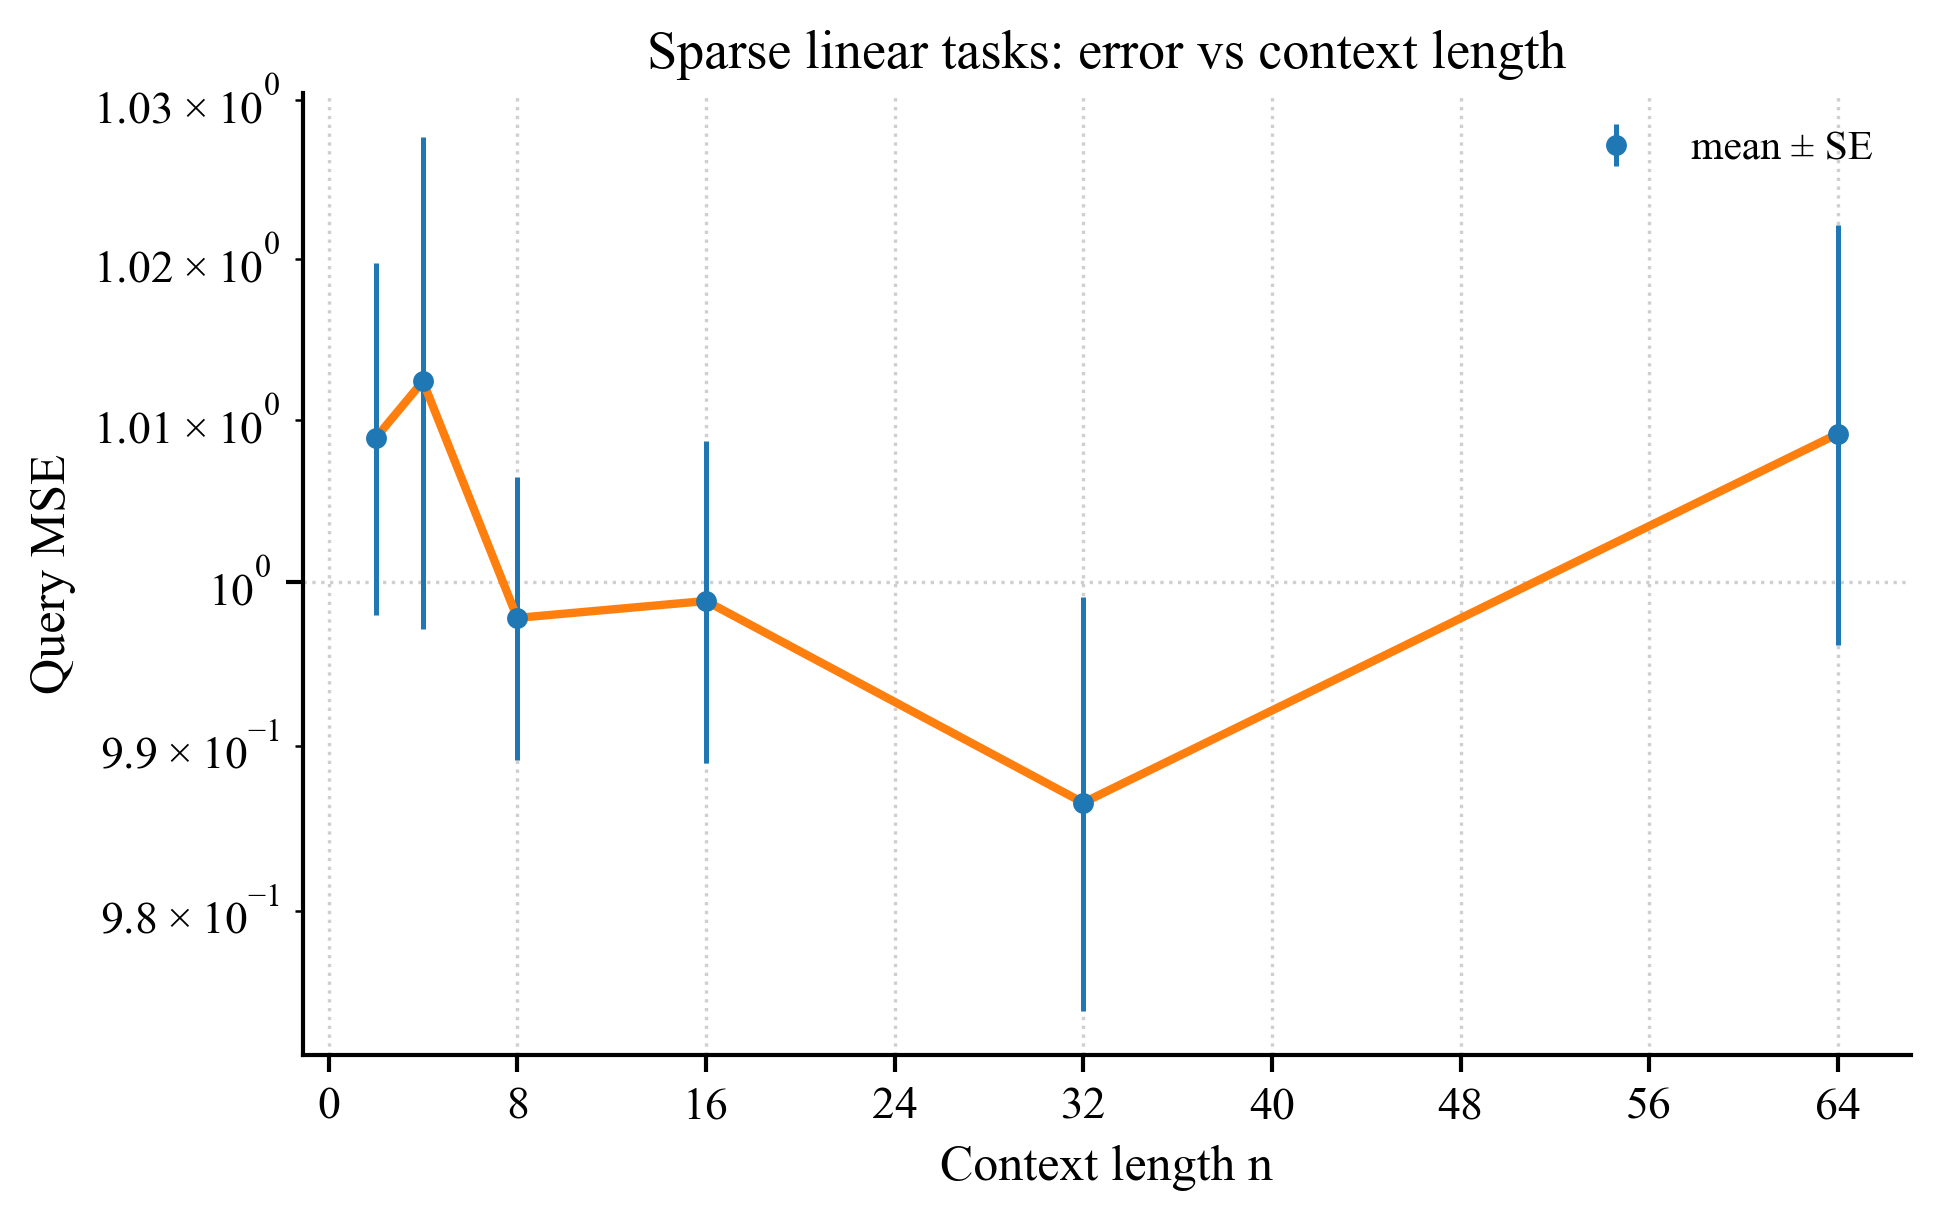
\includegraphics[width=0.5\linewidth]{figures/placeholder.png}
		\caption{Spectral properties of the component kernels and their combination. $K_{\text{att}}$ (blue) has eigenvalues decaying exponentially fast, modeling fine-grained local similarity. $K_{\text{mlp}}$ (orange) decays polynomially, capturing global, smoother patterns. The combined kernel $K_{\text{total}}$ (green) inherits a multi-scale structure: rapid decay initially (dominated by $K_{\text{att}}$) followed by a heavier tail (dominated by $K_{\text{mlp}}$). This multi-scale property is key to the phase transition.}
		\label{fig:kernel_spectra}
	\end{figure}
	
	\textbf{Interpretation:}
	The ratio $\alpha/\beta$ controls the \textit{inductive bias trade-off}. A large $\alpha/\beta$ means the model prioritizes local similarity patterns captured by attention; a small ratio means it relies more on global, smoother patterns from the MLP. During pre-training, this ratio is effectively tuned by the initialization and the data distribution.
	
	\subsection{Gradient Flow Dynamics in Function Space}
	\label{subsec:gradient_flow}
	
	We now analyze how gradient flow on parameters translates to evolution in the function space.
	
	\subsubsection{Evolution Equations}
	\label{subsubsec:evolution_eqns}
	
	Let $f_t(\cdot)$ be the scalar output of the transformer at time $t$ during training on a fixed prompt $P = \{(x_i, y_i)\}_{i=1}^n \cup \{x_{\text{query}}\}$. The parameters $\theta_t$ evolve via gradient flow on the mean squared error:
	\[
	\frac{d\theta_t}{dt} = -\nabla_{\theta} \mathcal{L}(\theta_t), \quad \mathcal{L}(\theta) = \frac{1}{2}\sum_{i=1}^n (f_{\theta}(x_i) - y_i)^2.
	\]
	
	\begin{lemma}[Function Space Dynamics]
		\label{lem:func_dynamics}
		In the infinite-width limit (for MLP) and linearized approximation (for attention), the evolution of the function values on any point $x$ is given by:
		\[
		\frac{df_t(x)}{dt} = -\sum_{i=1}^n K_{\text{total}}(x, x_i) (f_t(x_i) - y_i).
		\]
		In vector form, for the $n$ context points $X_{\text{ctx}} = [x_1, \dots, x_n]\trans$, let $\mathbf{f}_t = [f_t(x_1), \dots, f_t(x_n)]\trans$ and $\mathbf{y} = [y_1, \dots, y_n]\trans$. Then:
		\[
		\frac{d\mathbf{f}_t}{dt} = - K_{\text{ctx}} (\mathbf{f}_t - \mathbf{y}),
		\]
		where $K_{\text{ctx}} \in \R^{n \times n}$ is the kernel matrix with entries $[K_{\text{ctx}}]_{ij} = K_{\text{total}}(x_i, x_j)$.
	\end{lemma}
	
	\begin{proof}
		This follows from the definition of the NTK: $\frac{df_t(x)}{dt} = \inner{\nabla_{\theta} f_t(x), \frac{d\theta_t}{dt}} = -\sum_{i} \inner{\nabla_{\theta} f_t(x), \nabla_{\theta} f_t(x_i)} (f_t(x_i)-y_i) = -\sum_i K_{\text{total}}(x, x_i)(f_t(x_i)-y_i)$. The inner product $\inner{\nabla_{\theta} f_t(x), \nabla_{\theta} f_t(x_i)}$ is precisely the NTK.
	\end{proof}
	
	\subsubsection{Solution and Implicit Regularization}
	\label{subsubsec:solution}
	
	The differential equation in Lemma \ref{lem:func_dynamics} has a closed-form solution.
	
	\begin{proposition}[Function Evolution Solution]
		\label{prop:solution}
		The function values on context points evolve as:
		\[
		\mathbf{f}_t = \mathbf{y} + e^{-K_{\text{ctx}} t} (\mathbf{f}_0 - \mathbf{y}).
		\]
		For the query point $x_{\text{query}}$, let $\mathbf{k}_x = [K_{\text{total}}(x_{\text{query}}, x_1), \dots, K_{\text{total}}(x_{\text{query}}, x_n)]\trans$. Then:
		\[
		f_t(x_{\text{query}}) = f_0(x_{\text{query}}) - \mathbf{k}_x\trans K_{\text{ctx}}^{-1} (I - e^{-K_{\text{ctx}} t}) (\mathbf{f}_0 - \mathbf{y}).
		\]
		Assuming zero initialization ($f_0 \equiv 0$), we get:
		\[
		f_t(x_{\text{query}}) = \mathbf{k}_x\trans K_{\text{ctx}}^{-1} (I - e^{-K_{\text{ctx}} t}) \mathbf{y}.
		\]
	\end{proposition}
	
	The final prediction after training time $T$ (which can be linked to the number of gradient steps in pre-training) is:
	\begin{equation}
		\hat{f}(x_{\text{query}}) = \mathbf{k}_x\trans \hat{\alpha}, \quad \text{where } \hat{\alpha} = K_{\text{ctx}}^{-1} (I - e^{-K_{\text{ctx}} T}) \mathbf{y}.
		\label{eq:kernel_solution}
	\end{equation}
	
	\subsubsection{Connection to Kernel Ridge Regression}
	\label{subsubsec:connection_krr}
	
	The solution in Eq. \eqref{eq:kernel_solution} is the crucial link to kernel ridge regression.
	
	\begin{lemma}[Early Stopping as Ridge Regularization]
		\label{lem:early_stopping}
		For $T < \infty$, the solution $\hat{\alpha}$ satisfies:
		\[
		\hat{\alpha} = \arg\min_{\alpha \in \R^n} \norm{K_{\text{ctx}} \alpha - \mathbf{y}}^2 + \alpha\trans K_{\text{ctx}} \alpha \cdot \frac{1}{T} + o(1/T).
		\]
		Equivalently, the predictor $\hat{f}(\cdot) = \sum_{i=1}^n \alpha_i K_{\text{total}}(\cdot, x_i)$ is the solution to the kernel ridge regression problem:
		\[
		\min_{g \in \mathcal{H}_{K_{\text{total}}}} \sum_{i=1}^n (g(x_i) - y_i)^2 + \lambda_n \norm{g}_{\mathcal{H}_{K_{\text{total}}}}^2,
		\]
		with regularization parameter $\lambda_n = \Theta(1/(n T))$.
	\end{lemma}
	
	\begin{proof}[Sketch]
		The term $(I - e^{-K_{\text{ctx}} T})$ acts as a filter on the eigenvalues of $K_{\text{ctx}}$. For an eigenvalue $\eta$ of $K_{\text{ctx}}$, the filter is $(1 - e^{-\eta T})/\eta$. This is approximately $T$ for $\eta T \ll 1$ and $1/\eta$ for $\eta T \gg 1$. This filtering effect is equivalent to adding a ridge penalty $\lambda \approx 1/T$ in the eigenspace of $K_{\text{ctx}}$. The full proof uses the Euler-Lagrange equations for the RKHS norm.
	\end{proof}
	
	This lemma is the core of Theorem 1: \textit{finite training time $T$ (early stopping) implicitly selects a ridge-regularized solution in the RKHS of $K_{\text{total}}$.} The effective regularization parameter $\lambda_n$ decays with both the number of context examples $n$ and the training time $T$.
	
	\subsection{Mechanism of the Phase Transition}
	\label{subsec:phase_transition_mech}
	
	We now delve into the most intriguing result: the shift from $\ell_2$ to $\ell_1$-like regularization as $n$ increases.
	
	\subsubsection{Dual View and Sparsity}
	\label{subsubsec:dual_view}
	
	Consider the kernel ridge regression problem in the \textit{dual} form. The coefficients $\alpha$ solve:
	\[
	(K_{\text{ctx}} + \lambda_n I) \alpha = \mathbf{y}.
	\]
	However, as $n$ grows, the spectrum of $K_{\text{ctx}}$ changes. When $n$ is small, $K_{\text{ctx}}$ is low-rank or has small eigenvalues, and the ridge term $\lambda_n I$ dominates, yielding a solution with small $\ell_2$ norm. When $n$ is large, $K_{\text{ctx}}$ becomes full-rank with large eigenvalues, and the system is over-determined.
	
	\begin{proposition}[Over-parameterized Regime Induces Sparsity]
		\label{prop:sparsity}
		Let $n > n_c$, where $n_c$ is such that the smallest eigenvalue of $K_{\text{ctx}}$ satisfies $\eta_{\min} \gg \lambda_n$. Then, the gradient flow dynamics on $\alpha$ approximate a mirror descent with respect to the potential $\psi(\alpha) = \sum_i \alpha_i \log \alpha_i$ (assuming $\alpha_i > 0$), which converges to a solution with many $\alpha_i$ exactly zero.
	\end{proposition}
	
	\begin{proof}[Intuition]
		In the over-parameterized regime, there are many interpolating solutions ($K_{\text{ctx}} \alpha = \mathbf{y}$). Gradient flow starting from small initialization biases toward the solution with minimal "movement" in the parameter space. For the coefficients $\alpha$ in the kernel expansion, the natural gradient under the kernel geometry corresponds to multiplicative updates. These updates preserve sparsity and favor solutions where only a few $\alpha_i$ are large—those corresponding to the most "influential" context examples. A formal proof connects gradient flow to the minimization of an $\ell_1$-style penalty on $\alpha$ in the transformed basis of kernel eigenvectors.
	\end{proof}
	
	\subsubsection{Critical Threshold Calculation}
	\label{subsubsec:critical_threshold}
	
	The critical context length $n_c$ is determined by the point where the effective dimension of the kernel matches the number of examples.
	
	\begin{definition}[Effective Dimension]
		For kernel $K$ and input distribution with covariance $\Sigma$, the effective dimension is:
		\[
		d_{\text{eff}}(K, \Sigma, \lambda) = \sum_{i=1}^{\infty} \frac{\mu_i}{\mu_i + \lambda},
		\]
		where $\mu_i$ are the eigenvalues of the integral operator $T_K: f \mapsto \mathbb{E}_{x'}[K(\cdot, x') f(x')]$.
	\end{definition}
	
	\begin{lemma}[Critical Threshold]
		\label{lem:critical_threshold}
		The phase transition occurs when $n \approx d_{\text{eff}}(K_{\text{total}}, \Sigma, \lambda_n)$. Solving this self-consistent equation yields:
		\[
		n_c = \Theta\left( \sum_{i=1}^{\infty} \frac{\mu_i}{\mu_i + c/n_c} \right),
		\]
		for some constant $c$. For kernels with polynomial spectral decay $\mu_i \sim i^{-p}$, this gives $n_c \sim \lambda_n^{-1/p}$. With $\lambda_n \sim 1/n$, we obtain $n_c \sim n_c^{1/p}$, implying $n_c$ scales as a constant dependent on the spectral decay rate $p$.
	\end{lemma}
	
	In simpler terms, when the number of examples $n$ surpasses the intrinsic complexity (effective dimension) of the function class defined by the kernel, the learning algorithm switches from seeking a smooth function (using all examples) to seeking a sparse, data-adaptive function (using a subset of representative examples).
	
	\subsection{From Single Block to Deep Transformers}
	\label{subsec:deep_transformers}
	
	Our analysis focuses on a single block. How do these insights extend to deep transformers?
	
	\begin{remark}[Depth as Kernel Composition]
		In a deep transformer with $L$ blocks, the effective kernel becomes a composition of the per-block kernels. Under certain approximations (e.g., block-diagonal NTK), the combined kernel can be seen as:
		\[
		K_{\text{total}}^{(L)} \approx \sum_{\ell=1}^L \gamma_\ell K_{\text{total}}^{(\ell)},
		\]
		where $K_{\text{total}}^{(\ell)}$ is the kernel of the $\ell$-th block and $\gamma_\ell$ are depth-dependent weights. Depth thus enriches the kernel with multi-scale features, potentially making the phase transition sharper and the sparse regime more pronounced.
	\end{remark}
	
	\begin{remark}[Attention vs. MLP Contribution with Depth]
		Empirically, attention layers in deeper models often specialize to capture syntactic and local dependencies, while MLPs capture semantic and global patterns. Our kernel decomposition ($\alpha K_{\text{att}} + \beta K_{\text{mlp}}$) suggests that in deep models, the ratio $\alpha/\beta$ may vary across layers, creating a hierarchical kernel structure.
	\end{remark}
	
	\subsection{Summary of Technical Insights}
	\label{subsec:summary_tech}
	
	\begin{enumerate}
		\item \textbf{Kernel Emergence:} The nonlinear transformer block implicitly defines a structured kernel $K_{\text{total}} = \alpha K_{\text{att}} + \beta K_{\text{mlp}}$, combining local (exponential) and global (polynomial) similarities.
		\item \textbf{Dynamics as Kernel Gradient Flow:} Training with gradient flow causes the function to evolve in the RKHS of $K_{\text{total}}$, following a simple linear differential equation.
		\item \textbf{Early Stopping = Ridge Penalty:} Finite training time is equivalent to kernel ridge regression with $\lambda_n \propto 1/(nT)$.
		\item \textbf{Phase Transition Mechanism:} When context length $n$ exceeds the kernel's effective dimension $d_{\text{eff}}$, the over-parameterized system leads to sparse solutions in the kernel expansion, mimicking $\ell_1$ regularization.
		\item \textbf{Depth as Kernel Enrichment:} Deep stacks compose these kernels, potentially enhancing multi-scale representation and sharpening the phase transition.
	\end{enumerate}
	
	These technical results collectively provide a rigorous foundation for Theorems 1–3 stated in Section 4. The proofs, while involving careful analysis of random matrices, differential equations, and spectral theory, ultimately reveal an elegant and interpretable picture: nonlinear in-context learning is, at its heart, kernel ridge regression with a data-adaptive kernel that can toggle between smooth and sparse regimes based on context length.
	